Al calcular la matriz de potencial con el método de relajación sobre la región blanca se obtiene la gráfica \ref{fig:potencial}. Donde se aprecia que el potencial tiene un cambio menos drástico.

\begin{figure}[H]
\centering
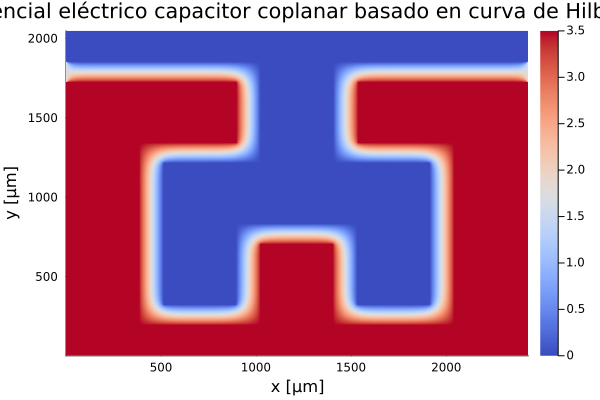
\includegraphics[width=1.1\columnwidth]{img/pothilheat.jpg}
    \caption{Potencial  }
    \label{fig:potencial}
\end{figure}

Para apreciar de mejor manera como cambia el potencial graficámos las lineas equipotenciales donde es claro que siguen el contorno de los electrodos, con suavización en las esquinas, donde hay efectos de borde.  

\begin{figure}[H]
\centering
    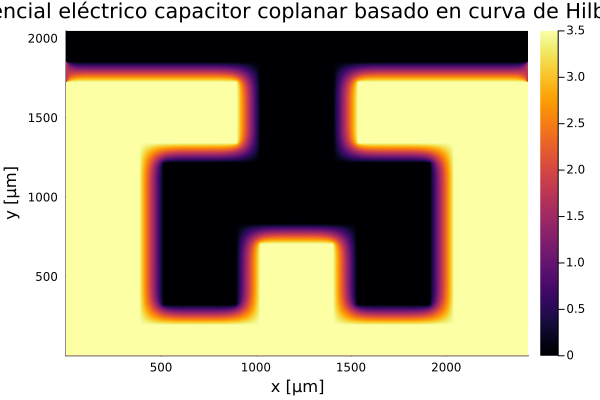
\includegraphics[width=1.2\columnwidth]{img/pothileq.jpg}
    \caption{Lineas equipotenciales  }
    \label{fig:equipV}
\end{figure}

La gráfica del campo eléctrico muestra, lineas son perpendiculares a las lineas equipotenciales, van del cátodo positivo al negativo, lo que indica la precensia de carga positiva y negativa, pues las líneas de campo nacen en las positivas y mueren en las negativas.  


\begin{figure}[H]
\centering
    \includegraphics[width=1.2\columnwidth]{img/Campo.jpg}
    \caption{Campo eléctrico}
    \label{fig:equipV}
\end{figure}

Finalmente al calcular la densidad de carga se obtiene la gráfica, donde podemos apreciar que la carga positiva se acumula en el electrodo con volteje positivo y positiva en el electrodo con voltaje 0.  

\begin{figure}[H]
\centering
    \includegraphics[width=1.2\columnwidth]{}
    \caption{Distribucion de carga}
    \label{fig:equipV}
\end{figure}

Al sumar la carga positiva en se obtiene $Q= 1000 pesos $ y la diferencia de voltaje es 3.5 con lo que la capacitancia es $C=\frac{Q}{\Delta\phi}$